\documentclass[11pt]{article}

\usepackage[letterpaper,margin=0.88in,headheight=15pt]{geometry}
\usepackage{microtype}
\usepackage{amsmath,amssymb,mathtools}
\usepackage{booktabs,tabularx,array}
\usepackage{graphicx}
\usepackage{xcolor}
\usepackage{hyperref}
\usepackage{url}
\usepackage{xspace}
\usepackage{fancyhdr}
\usepackage{caption}
\usepackage{float}
\usepackage{pgfplots}
\usepackage{pgfplotstable}
\usepackage{tikz}
\usepackage{siunitx}
\usepackage{lastpage}

\pgfplotsset{compat=1.18}
\graphicspath{{figures/}}

\definecolor{ink}{HTML}{1C2430}
\definecolor{muted}{HTML}{5F6B7A}
\definecolor{rulegray}{HTML}{D7DCE2}
\definecolor{blue}{HTML}{356AA0}
\definecolor{gold}{HTML}{C8932D}
\definecolor{orange}{HTML}{D66A2C}
\definecolor{paleblue}{HTML}{EEF4FA}

\hypersetup{
  colorlinks=true,
  linkcolor=blue,
  citecolor=blue,
  urlcolor=blue,
  pdftitle={Why Does ESMFold2 Keep ESMC State 51?},
  pdfauthor={Synthyra Research},
  pdfsubject={A weights-only investigation of a transient folding interface in ESMC-6B}
}

\pagestyle{fancy}
\fancyhf{}
\fancyhead[L]{\footnotesize\color{muted}Why does ESMFold2 keep ESMC state 51?}
\fancyhead[R]{\footnotesize\color{muted}ESMC-6B weight geometry}
\fancyfoot[L]{\footnotesize\color{muted}Synthyra Research}
\fancyfoot[R]{\footnotesize\color{muted}\thepage\ of \pageref{LastPage}}
\renewcommand{\headrulewidth}{0.4pt}
\renewcommand{\footrulewidth}{0pt}
\fancypagestyle{firstpage}{%
  \fancyhf{}
  \fancyfoot[L]{\footnotesize\color{muted}Synthyra Research}
  \fancyfoot[R]{\footnotesize\color{muted}\thepage\ of \pageref{LastPage}}
  \renewcommand{\headrulewidth}{0pt}
  \renewcommand{\footrulewidth}{0pt}
}

\captionsetup{font=small,labelfont=bf,textfont={color=muted}}
\sisetup{detect-all,round-mode=places,round-precision=3}
\setlength{\parindent}{1.25em}
\setlength{\parskip}{0.32em}
\setlength{\emergencystretch}{2em}

\newcommand{\ESMC}{ESMC-6B\xspace}
\newcommand{\ESMFold}{ESMFold2\xspace}
\newcommand{\R}{\mathbb{R}}
\newcommand{\mat}[1]{\mathbf{#1}}
\newcommand{\vect}[1]{\boldsymbol{#1}}

\pgfplotsset{
  report axis/.style={
    width=\textwidth,
    height=0.46\textwidth,
    axis line style={draw=ink!70},
    tick style={draw=ink!65},
    tick label style={font=\footnotesize,color=muted},
    label style={font=\small,color=ink},
    grid=major,
    grid style={draw=rulegray!70,line width=0.2pt},
    legend style={font=\footnotesize,draw=none,fill=none,cells={anchor=west}},
    every axis plot/.append style={line width=1.15pt},
    clip=true
  }
}

\begin{document}

\thispagestyle{firstpage}
\noindent{\color{blue}\rule{\textwidth}{1.8pt}}\\[0.55cm]
{\LARGE\bfseries\color{ink} Why does ESMFold2 keep ESMC state 51?\par}
\vspace{0.18cm}
{\large\color{muted} A weights-only search for a transient folding interface inside a protein language model\par}
\vspace{0.45cm}
\noindent{\small\color{muted}Synthyra Research \hfill July 28, 2026}
\vspace{0.45cm}

The recent \ESMC paper pushed data and architecture scaling further for protein masked-language modeling, and one of its most interesting results is how clearly structural information changes across the depth of the network \cite{candido2026}. This continues a pattern from earlier protein language models. Sequence-only ESM representations supported probes for secondary structure, residue contacts, and protein function \cite{rives2021}, while particular attention heads recovered residue-residue contacts without ever being trained on contact labels \cite{rao2021}. As those representations became stronger, it became natural to attach a folding model that could learn how to use them directly, first in ESMFold and now in \ESMFold \cite{lin2023}.

The layer-wise results in the \ESMC paper make that connection especially interesting. Long-range contact precision remains low through much of the 80-block network and then climbs sharply near the end. The paper reports this as P@L, meaning precision among the top $l$ predicted contacts for a protein of length $l$. The uppercase letter is retained in the conventional metric name, while sequence length is the lowercase scalar $l$ in the mathematics here. For a 300-residue protein, if 210 of the 300 highest-scoring residue pairs are true long-range contacts, P@L is $210/300=0.70$. In practical terms, the metric asks whether a layer makes it easy to identify residues that are far apart in sequence but close together in three-dimensional structure.

\begin{figure}[H]
\centering
\includegraphics[width=0.58\textwidth]{published_figure1d.png}
\caption{The published \ESMC depth profile. Long-range contact P@L, in teal, remains low through the early network and rises sharply in later states. EC-class neighborhood accuracy, in purple, peaks earlier. Reproduced from panel D of Figure 1 in Candido et al. under CC BY 4.0 \cite{candido2026}.}
\label{fig:published-pal}
\end{figure}

The steady improvement toward the end of the network fits the usual picture in which early blocks handle more local sequence relationships and later blocks integrate those relationships over longer ranges. This does not require the final state to contain every structural fact in some absolute sense. It only says that a relatively simple contact readout can access tertiary structure more cleanly there. We became interested in what happens when the downstream consumer is not a contact probe but \ESMFold itself. Because the folding model learns a mixture over the full ESMC depth, the P@L trend led us to expect most of the mixture to accumulate on later states, with relatively little reason to preserve an isolated intermediate state.

To see whether that expectation holds, it helps to make the interface explicit. \ESMC exposes 81 states, with state 0 representing the token embedding before any transformer block and states 1 through 80 representing the outputs of blocks 0 through 79. For batch size $b$, sequence length $l$, and hidden width 2560, the complete stack is the tensor
\[
\mat{H}\in\R^{b\times81\times l\times2560}.
\]
Passing all 81 states at full width into the folding trunk would be unwieldy. Instead, \ESMFold normalizes every state with one shared LayerNorm, projects it from 2560 channels to 256 channels with one shared matrix $\mat{W}_{P}\in\R^{256\times2560}$, and then learns one scalar logit $c_s$ for each state $s$. A softmax turns those logits into positive mixing masses that sum to one,
\begin{equation}
a_s=\frac{\exp(c_s)}{\sum_{t=0}^{80}\exp(c_t)},
\qquad \sum_{s=0}^{80}a_s=1.
\label{eq:mixer}
\end{equation}
The tensor passed into the folding trunk is
\begin{equation}
\mat{Z}=\sum_{s=0}^{80}a_s\,\mathcal{N}(\mat{H}_s)\mat{W}_{P}^{\mathsf T}
\in\R^{b\times l\times256}.
\label{eq:foldinput}
\end{equation}
Because normalization and projection are shared across depth, \ESMFold is not learning 81 separate interpretations of the residual stream. It applies the same 256-dimensional reader to every state and learns how much of each projected state to retain. This makes the coefficients informative about preference, although not about a literal fraction of folding information. A value such as $a_{51}=0.10$ means that state 51 receives one tenth of the convex mixing mass, but two projected states can be redundant, complementary, different in norm, or partially canceling. The coefficient therefore tells us that optimization consistently retained state 51, not that removing it would reduce folding accuracy by ten percent.

When we extracted the coefficients from all four \ESMFold checkpoints supported by FastPLMs, the broad result followed the P@L trend. The final four states account for 60.44\% to 65.41\% of the total mass, and the complete 81-state profiles are extremely similar across checkpoints. Pairwise Pearson correlations range from 0.988 to 0.997, while pairwise Spearman correlations range from 0.981 to 0.996.

\begin{figure}[H]
\centering
\begin{tikzpicture}
\begin{axis}[
  report axis,
  xlabel={ESMC hidden-state index},
  ylabel={softmax mixing mass (\%)},
  xmin=0,xmax=80,
  ymin=0,ymax=27,
  legend columns=2,
  legend pos=north west,
  extra x ticks={51},
  extra x tick labels={},
]
\addplot[blue] table[x=state,y=weight]{figures/mixer_esmfold2.dat};
\addlegendentry{ESMFold2}
\addplot[orange,dashed] table[x=state,y=weight]{figures/mixer_experimental_fast.dat};
\addlegendentry{Experimental Fast 2025}
\addplot[gold,dashdotted] table[x=state,y=weight]{figures/mixer_experimental.dat};
\addlegendentry{Experimental 2025}
\addplot[ink!75,dotted] table[x=state,y=weight]{figures/mixer_fast.dat};
\addlegendentry{ESMFold2 Fast}
\draw[dashed,ink!75] (axis cs:51,0) -- (axis cs:51,27);
\node[anchor=west,font=\footnotesize,color=muted] at (axis cs:51.7,21){state 51};
\end{axis}
\end{tikzpicture}
\caption{The four learned layer mixtures. All are dominated by the final states, but every checkpoint also preserves a sharp state-51 peak.}
\label{fig:mixer}
\end{figure}

We also wanted to make the relationship with P@L visible rather than leaving it as a correlation coefficient in the text. The underlying source-data table for Figure 1D was not distributed with our weight archive, but the plotted markers are stored as vector paths in the paper PDF. We read those marker coordinates directly and mapped the vertical axis back to the reported P@L scale. This recovers 80 figure-derived values for transformer blocks 0 through 79 without tracing a raster image. Since block $b$ produces state $b+1$, each P@L value was paired with the coefficient $a_{b+1}$ from the folding mixture.

The four-checkpoint mean gives Pearson $r=0.635$ and Spearman $\rho=0.655$, while the individual-checkpoint values range from 0.625 to 0.645 for Pearson and from 0.629 to 0.673 for Spearman. The correlation reflects the shared rise near the end of the model, but the scatter also makes the intermediate mismatch clear. State 51 receives a mean mixing mass of 10.26\% even though block 50 has P@L of only about 0.092. Relative to a simple linear fit, state 51 has the third-largest positive residual in the network, exceeded only by states 79 and 80.

\begin{figure}[H]
\centering
\begin{minipage}[t]{0.49\textwidth}
\centering
\begin{tikzpicture}
\begin{axis}[
  width=\linewidth,
  height=0.76\linewidth,
  xlabel={transformer block},
  ylabel={value (\%)},
  xmin=0,xmax=79,
  ymin=0,ymax=75,
  tick label style={font=\scriptsize,color=muted},
  label style={font=\footnotesize,color=ink},
  title style={font=\footnotesize,color=ink},
  title={Depth profiles},
  grid=major,
  grid style={draw=rulegray!70,line width=0.2pt},
  legend style={font=\scriptsize,draw=none,fill=none,at={(0.02,0.98)},anchor=north west},
]
\addplot[blue,line width=1.1pt] table[x=block,y=pal_pct]{figures/pal_mixer_comparison.dat};
\addlegendentry{P@L $\times100$}
\addplot[orange,line width=1.1pt] table[x=block,y=mean]{figures/pal_mixer_comparison.dat};
\addlegendentry{mean mixing mass}
\draw[dashed,ink!65] (axis cs:50,0) -- (axis cs:50,75);
\node[anchor=west,font=\scriptsize,color=ink] at (axis cs:50.8,65){state 51};
\end{axis}
\end{tikzpicture}
\end{minipage}\hfill
\begin{minipage}[t]{0.49\textwidth}
\centering
\begin{tikzpicture}
\begin{axis}[
  width=\linewidth,
  height=0.76\linewidth,
  xlabel={P@L of producing block},
  ylabel={mean mixing mass (\%)},
  xmin=0,xmax=0.75,
  ymin=0,ymax=25,
  tick label style={font=\scriptsize,color=muted},
  label style={font=\footnotesize,color=ink},
  title style={font=\footnotesize,color=ink},
  title={Layer-wise association},
  grid=major,
  grid style={draw=rulegray!70,line width=0.2pt},
]
\addplot[only marks,mark=*,mark size=1.35pt,draw=blue!70,fill=blue!45]
  table[x=pal,y=mean]{figures/pal_mixer_comparison.dat};
\addplot[only marks,mark=*,mark size=2.4pt,draw=orange,fill=orange]
  coordinates {(0.09223054,10.2571086076)};
\node[anchor=west,font=\scriptsize,color=ink] at (axis cs:0.105,10.3){state 51};
\node[anchor=west,font=\scriptsize,color=ink,align=left] at (axis cs:0.04,23.0){Pearson 0.635\\Spearman 0.655};
\end{axis}
\end{tikzpicture}
\end{minipage}
\caption{P@L and learned layer contribution share a broad depth trend. The left panel overlays the figure-derived P@L values with the mean mixing profile. The right panel pairs each block's P@L with the mean contribution of the state it produces. State 51 is the conspicuous intermediate-depth outlier.}
\label{fig:pal-mixer}
\end{figure}

The unexpected part of the mixture is the narrow peak at state 51. It receives 9.99\%--10.65\% of the total mass and ranks fourth in every checkpoint, making it a reproducible secondary component rather than a small coefficient left behind after training. The peak is particularly notable because the surrounding P@L values do not suggest that this part of the network should compete with the final states.

\begin{table}[H]
\centering
\caption{Exact state-51 and late-state mixing masses. Values are fractions of the 81-state softmax total.}
\label{tab:mixer}
\begin{tabular}{@{}lrrrr@{}}
\toprule
Checkpoint & $a_{51}$ & Rank & Mass 77--80 & Effective states \\
\midrule
ESMFold2 & 0.10654 & 4 & 0.65412 & 10.64 \\
Experimental 2025 & 0.09988 & 4 & 0.60439 & 11.46 \\
Experimental Fast 2025 & 0.10253 & 4 & 0.62210 & 10.86 \\
ESMFold2 Fast & 0.10134 & 4 & 0.63480 & 10.79 \\
\bottomrule
\end{tabular}
\end{table}

The effective-state count in the last column gives another way to describe how selective the mixture is. If equal mass were placed on exactly $n$ states, the entropy of the mixture would correspond to $n$ effective states. Formally, with masses $a_s$,
\begin{equation}
n_{\mathrm{eff}}=\exp\!\left(-\sum_{s=0}^{80}a_s\log a_s\right).
\end{equation}
Values near 11 mean that the nominal 81-state mixture behaves more like a focused mixture over roughly eleven equally weighted states, with state 51 firmly inside that selected set. This raised another question about the results already reported in the \ESMC paper. The authors had trained sparse autoencoders to study how the internal representation changes with depth, and their layer-wise curves showed a pronounced feature in the same part of the network.

A sparse autoencoder, or SAE, tries to reconstruct a model state through a much larger dictionary while allowing only a small number of dictionary features to be active at once. The authors trained a separate TopK SAE on the per-amino-acid hidden vectors from every layer of the final \ESMC checkpoint. Each input vector was standardized, mapped into a nonnegative feature code, reduced to its $k$ largest activations, and decoded back into the original 2560-dimensional space. Training used eight billion tokens drawn from the same clustered UniRef, MGnify, and JGI distribution used for the language model. For the layer-wise comparison in Figure S26, they evaluated codebooks with 16,384 and 131,072 features.

If $\vect{h}_s$ is the hidden vector from state $s$ and $\widehat{\vect{h}}_s$ is the SAE reconstruction, the reported reconstruction term is the mean squared difference across the $d$ hidden channels,
\begin{equation}
\ell_{\mathrm{recon},s}=\frac{1}{d}\left\|\widehat{\vect{h}}_s-\vect{h}_s\right\|_2^2.
\end{equation}
The authors also replaced each original layer state with its SAE reconstruction, continued the forward pass, and measured the change in full-sequence masked-language-model perplexity. Reconstruction loss measures how much of the vector the sparse dictionary fails to reproduce, while perplexity degradation measures whether the missing part matters to masked-token prediction. Figure S26 plots reconstruction loss for both codebook sizes and perplexity degradation for the 16,384-feature SAE.

Both curves dip around layers 48--51 and become much larger through layers 60--70. The state that receives a large folding coefficient is therefore neither the strongest contact state nor the state whose sparse reconstruction most disrupts the language model. The authors describe the two SAE measurements as proxies for information density, but for our question the important point is more specific. Contact precision, sparse reconstruction, masked-token prediction, and folding can prefer different directions within the same hidden vector.

\begin{figure}[H]
\centering
\includegraphics[width=\textwidth]{published_figure_s26.png}
\caption{Published Figure S26 from Candido et al. \cite{candido2026}. SAE reconstruction loss and perplexity degradation both dip near layers 48--51 and rise later. Reproduced under CC BY 4.0. These activation-based curves provide context for the question and were not regenerated in this weights-only analysis.}
\label{fig:published-s26}
\end{figure}

Each diagnostic applies a different operation to the same high-dimensional state. P@L asks whether a contact-oriented readout can recover residue pairs. The SAE asks whether a sparse dictionary can reconstruct the state while preserving masked-language-model behavior. \ESMFold first restricts the state to the row space of its learned 256-dimensional projection. A direction can matter strongly to that projection while contributing little to contact precision or SAE reconstruction error. We therefore moved away from the broad claim that state 51 contains more information and considered whether block 50 might write directions that the folding projection is particularly well suited to read.

The hypothesis depends on the state-to-block indexing because state 0 is the embedding, so if transformer block $b$ implements the map $\mathcal{T}_b$, then
\begin{equation}
\mat{H}_{b+1}=\mathcal{T}_b(\mat{H}_b),
\qquad b\in\{0,\ldots,79\}.
\label{eq:indexing}
\end{equation}
Consequently,
\[
\mat{H}_{51}=\mathcal{T}_{50}(\mat{H}_{50}).
\]
This means that block 50 produces state 51, whereas block 51 consumes state 51 and produces state 52. Any feature that first becomes available in state 51 must have been written by block 50, although block 51 may subsequently preserve, transform, or remove it. We therefore treated block 50 as the primary candidate and block 51 as an adjacent control throughout the analysis.

For this pass we deliberately restricted the evidence to checkpoint weights. We did not pass sequences through \ESMC or generate hidden states, attention maps, SAE activations, folds, or biological outputs. This prevents us from claiming that the candidate pathway is used on real proteins, but it still allows us to ask whether the operators in block 50 make an unusually direct route into the folding projection available.

Each transformer block supplies two broad paths, with attention moving information among residue positions and a SwiGLU feed-forward network transforming each position independently before writing back to the residual stream. Attention contains query, key, value, and output matrices, all with hidden width 2560. The checkpoint stores query, key, and value as one $7680\times2560$ matrix, which we split into
\[
\mat{W}_Q,\mat{W}_K,\mat{W}_V\in\R^{2560\times2560}.
\]
The attention output matrix is $\mat{W}_O\in\R^{2560\times2560}$. The SwiGLU path expands from 2560 channels to 6912 intermediate neurons using a gate matrix $\mat{W}_G$ and a value matrix $\mat{W}_U$, both in $\R^{6912\times2560}$, then returns through $\mat{W}_D\in\R^{2560\times6912}$. LayerNorm weights, biases, and query/key normalization vectors were measured separately. We repeated the same inventory for all 80 blocks so that block 50 would always be judged against the rest of the network rather than in isolation.

Since the folding projection keeps only 256 of the 2560 residual channels, the first possibility we checked was whether block 50 had already compressed the residual stream into an unusually low-dimensional form. If so, the large state-51 coefficient might only reflect a generic bottleneck that happened to fit inside the folding input. Singular value decomposition gives a direct way to test that possibility from the weights.

For any matrix $\mat{W}\in\R^{m\times n}$, singular value decomposition writes
\begin{equation}
\mat{W}=\mat{U}\mat{\Sigma}\mat{V}^{\mathsf T}.
\label{eq:svd}
\end{equation}
The columns of $\mat{V}$ are orthogonal input directions, the columns of $\mat{U}$ are the corresponding output directions, and the diagonal entries $\sigma_1\ge\sigma_2\ge\cdots\ge0$ of $\mat{\Sigma}$ say how strongly the matrix acts along each pair. A matrix with one large singular value and many tiny ones behaves almost like a one-dimensional operator, while a matrix with many comparable singular values acts substantially along many independent directions.

The matrices here are large enough that it is useful to recall why a Gram matrix appears. Multiplying $\mat{W}$ by its transpose gives
\begin{align}
\mat{W}^{\mathsf T}\mat{W}
&=\mat{V}\mat{\Sigma}^2\mat{V}^{\mathsf T}, \\
\mat{W}\mat{W}^{\mathsf T}
&=\mat{U}\mat{\Sigma}^2\mat{U}^{\mathsf T}.
\end{align}
These are Gram matrices, which means that every entry is an inner product between two columns or two rows of $\mat{W}$. Their eigenvectors recover the singular directions and their eigenvalues are $\sigma_i^2$. Computing the smaller Gram matrix saves memory for a rectangular weight matrix without changing the singular spectrum. We accumulated it in FP64 because the smallest eigenvalues are particularly sensitive to rounding. A true Gram matrix cannot have negative eigenvalues, although floating-point arithmetic can produce tiny negative values near zero. We clamped only those numerical negatives and recorded their total magnitude.

Before comparing spectral summaries, it is worth making the word ``energy'' precise because it can otherwise sound more mysterious than it is. In matrix analysis, energy is conventional shorthand for the sum of squared entries. It is not physical energy, biological activity, or a measurement of how much information the model uses. For a weight matrix $\mat{W}$, this quantity is the squared Frobenius norm
\begin{equation}
e(\mat{W})=\|\mat{W}\|_F^2
=\sum_{i,j}w_{ij}^2
=\sum_i\sigma_i^2
\end{equation}
which adds the squared value of every entry. The same total can be computed by adding the squared singular values, so each $\sigma_i^2$ tells us how much of the matrix's squared magnitude belongs to singular direction $i$. Squaring prevents positive and negative weights from cancelling one another, much as variance squares deviations from a mean, and orthogonal singular directions then add without cross terms. A statement such as ``rank 128 retains 90\%'' therefore has a literal meaning. The first 128 singular directions reproduce 90\% of the sum of squared weights, leaving 10\% as squared reconstruction error. It does not mean that they preserve 90\% of folding accuracy, biological information, or model behavior, none of which can be inferred without running the model.

No single scalar captures the whole shape of a spectrum, so we used several summaries that answer slightly different questions. Stable rank measures the total squared magnitude in units of the strongest singular direction,
\begin{equation}
\operatorname{srank}(\mat{W})=
\frac{\|\mat{W}\|_F^2}{\|\mat{W}\|_2^2}
=\frac{\sum_i\sigma_i^2}{\sigma_1^2}.
\end{equation}
If every active direction were as strong as $\sigma_1$, stable rank would equal the number of active directions. A value of 17 therefore means that the matrix contains the same total squared magnitude as roughly seventeen copies of its strongest direction. The quantity is unchanged if the whole matrix is rescaled, but it is strongly influenced by the largest singular value. One dominant direction can keep stable rank low even when a long tail of weaker directions is still important.

Participation ratio and entropy-based effective rank begin by converting each squared singular value into its fraction of the total,
\begin{equation}
p_i=\frac{\sigma_i^2}{\sum_j\sigma_j^2}.
\end{equation}
They then summarize how evenly those fractions are distributed,
\begin{align}
\operatorname{PR}(\mat{W})&=\frac{1}{\sum_i p_i^2},\\
\operatorname{erank}(\mat{W})&=\exp\!\left(-\sum_i p_i\log p_i\right).
\end{align}
Both expressions return $n$ when exactly $n$ directions carry equal fractions and return a value near one when a single direction dominates. Effective rank first computes the Shannon entropy of the full distribution and then asks how many equally weighted directions would have the same entropy \cite{roy2007}. Participation ratio gives more influence to the largest fractions because each $p_i$ is squared, so it is less forgiving of a sharply concentrated top spectrum. Stable rank is more top-heavy still because it compares everything directly with $\sigma_1^2$. Reading the three together tells us whether a matrix has one unusually strong direction, a compact group of strong directions, or a broad tail spread across hundreds of weaker directions. We also measured the number of singular vectors needed to retain 90\%, 95\%, and 99\% of the squared Frobenius magnitude and the reconstruction error at ranks 16 through 2048.

This uncentered spectrum describes the matrix as a linear operator. We also ran row- and column-PCA after subtracting the relevant mean vector. The centered analysis asks how many directions describe variation among learned neurons. An operator may have a large common component that dominates uncentered SVD but disappears after centering, so agreement between the two views is more persuasive than either alone.

These measurements did not show a low-dimensional bottleneck at block 50. Its query matrix $\mat{W}_Q$ has effective rank 718.51, participation ratio 175.08, stable rank 17.23, and a leading squared-magnitude fraction of 0.0580. The last two numbers are the same fact viewed from opposite directions because $1/0.0580\approx17.24$. The strongest direction accounts for 5.8\% of the total, which is enough to pull stable rank down to about 17, while the remaining 94.2\% is distributed across a long tail that keeps effective rank above 700. The matrix is spectrally uneven, but it has not collapsed into a small global subspace.

\begin{figure}[H]
\centering
\begin{tikzpicture}
\begin{axis}[
  report axis,
  xlabel={ESMC transformer block},
  ylabel={Q effective rank},
  xmin=0,xmax=79,
  ymin=0,ymax=1750,
]
\addplot[blue] table[x=block,y=effective_rank]{figures/q_effective_rank.dat};
\draw[dashed,orange] (axis cs:50,0) -- (axis cs:50,1750);
\node[anchor=west,font=\footnotesize,color=ink] at (axis cs:50.7,1540){block 50};
\end{axis}
\end{tikzpicture}
\caption{Effective rank of the query matrix across depth. Rank changes strongly and smoothly across the network, but block 50 is not a singular low-rank collapse.}
\label{fig:qrank}
\end{figure}

Much of the spectral movement is explained by depth because, after subtracting a smooth cubic trend, mixer mass is inversely associated with query participation ratio ($r\approx-0.757$), query effective rank ($r\approx-0.672$), key effective rank ($r\approx-0.675$), and query stable rank ($r\approx-0.561$). Later states with larger folding coefficients therefore tend to be produced by spectrally more concentrated attention operators. The association is broad rather than specific to block 50 because the query-effective-rank correlation remains between $-0.567$ and $-0.489$ when the profiles are shifted by lags from $-2$ through $+2$.

We kept several additional spectral-shape measurements because two matrices can have similar effective ranks while distributing their largest singular values differently. The first quantity in Figure~\ref{fig:spectralshape} is the fraction of squared Frobenius magnitude captured by the leading 16 directions,
\begin{equation}
e_{16}=\frac{\sum_{i=1}^{16}\sigma_i^2}{\sum_j\sigma_j^2}.
\end{equation}
A value of 0.20 means that 20\% of the total squared weight magnitude lies in those 16 directions.

The spectral Gini coefficient asks a different and deliberately simple question. If the singular-value magnitude were divided among the available directions, how unequal would that division be? For $n$ nonnegative values, it can be written as the average absolute difference across every pair, normalized by the total magnitude,
\begin{equation}
g(\vect{x})=
\frac{\sum_{i=1}^{n}\sum_{j=1}^{n}|x_i-x_j|}
{2n\sum_{i=1}^{n}x_i}.
\end{equation}
Every pairwise difference vanishes when the values are equal, which gives $g=0$. If one value contains everything and the other $n-1$ values are zero, then $g=(n-1)/n$, which approaches one as $n$ grows. The four-value examples $(1,1,1,1)$ and $(4,0,0,0)$ consequently have Gini coefficients of 0 and 0.75. For spectral Gini we substitute $x_i=\sigma_i$, so a high value means that a small set of singular directions has much larger gain than the rest. We intentionally use $\sigma_i$ rather than $\sigma_i^2$ here. Effective rank already describes the distribution of squared magnitude, while Gini gives a less top-heavy view of inequality among the singular values themselves.

The power-law head slope describes how quickly the leading spectrum falls by fitting
\begin{equation}
\log\sigma_i\approx a+\beta\log i
\end{equation}
over ranks 16 through 256. A more negative scalar $\beta$ means that singular values shrink more quickly as rank increases. We estimated a descriptive knee rank by joining the first and last points of the log spectrum with a straight line and selecting the rank with the largest normalized departure from that line. A boundary value near the full rank usually means that no clear interior knee was found, which explains the abrupt jumps in the lower-right panel and is why knee rank was treated as a diagnostic rather than a primary inferential result.

\begin{figure}[H]
\centering
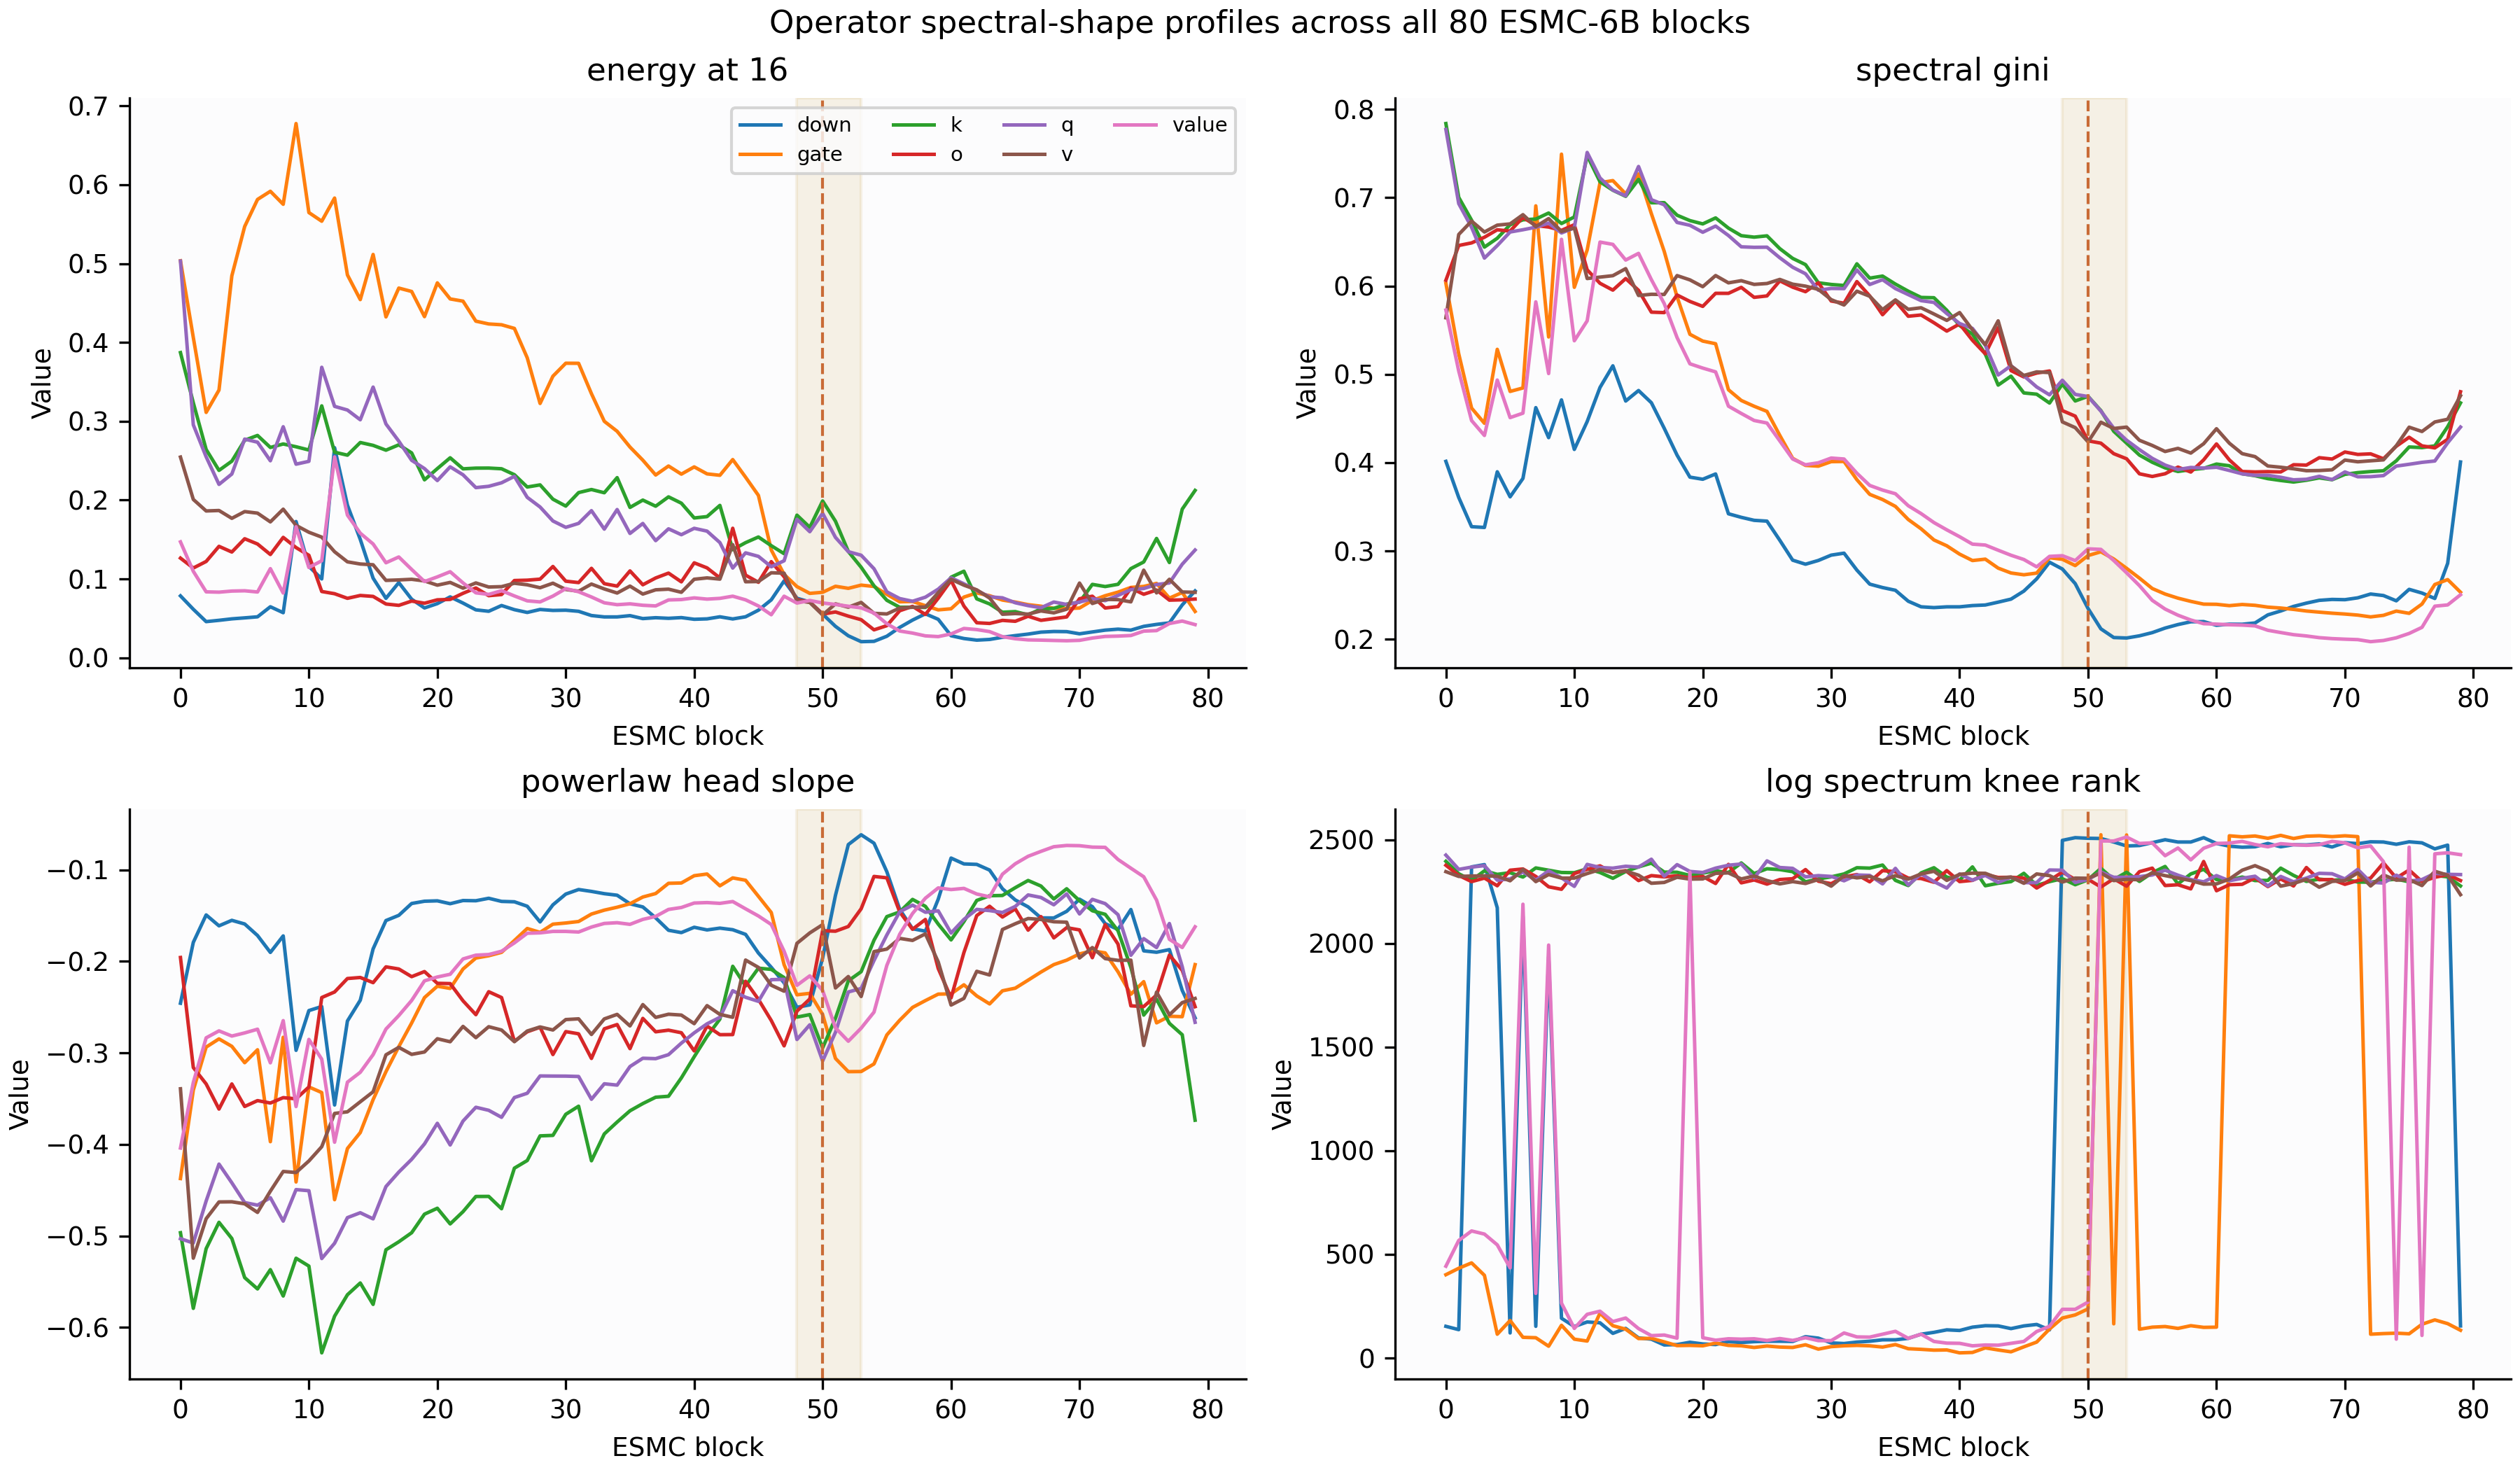
\includegraphics[width=\textwidth]{spectral_shape_profiles.png}
\caption{Top-16 squared magnitude, labeled ``energy at 16,'' singular-value Gini, head slope, and knee rank across the seven matrix families. Blocks 48--53 are shaded and block 50 is dashed. No family undergoes a unique whole-matrix rank collapse at block 50.}
\label{fig:spectralshape}
\end{figure}

Once a global low-rank bottleneck had been ruled out, the more relevant comparison was between block 50 and the particular downstream model that selected it. The first learned \ESMFold operation is the shared projection $\mat{W}_P$, whose 256 rows span the directions in the 2560-dimensional residual stream that can survive into the folding trunk while every orthogonal direction is discarded. This shifted the analysis from absolute simplicity to compatibility with the folding reader. We asked whether the most prominent directions in block 50 were unusually aligned with the 256-dimensional row space of $\mat{W}_P$.

For input-side matrices such as $\mat{W}_Q$, $\mat{W}_K$, $\mat{W}_V$, $\mat{W}_G$, and $\mat{W}_U$, the right singular vectors in $\mat{V}$ identify residual-stream directions that the operator reads. For output matrices such as $\mat{W}_O$ and $\mat{W}_D$, the left singular vectors in $\mat{U}$ identify residual-stream directions that the operator writes. Let $\mat{U}_r\in\R^{2560\times r}$ contain the leading $r$ residual-coordinate directions from one of those operators, and let $\mat{P}\in\R^{2560\times256}$ be an orthonormal basis for the row space of $\mat{W}_P$. Their normalized overlap is
\begin{equation}
o_r(\mat{U}_r,\mat{P})
=\frac{\|\mat{U}_r^{\mathsf T}\mat{P}\|_F^2}{r}
=\frac{1}{r}\sum_{i=1}^{r}\cos^2\theta_i,
\label{eq:overlap}
\end{equation}
where $\theta_i$ are principal angles between the two subspaces. The overlap is one when every direction in $\mat{U}_r$ lies inside the folding row space and zero when the spaces are orthogonal. For a random rank-$r$ subspace in 2560 dimensions compared with a 256-dimensional projection, the expected overlap is simply
\begin{equation}
\mathbb{E}[o_r]=\frac{256}{2560}=0.10.
\end{equation}
The random expectation matters because unrelated high-dimensional subspaces still overlap by chance. An observed value of 0.16 does not mean that a subspace contains 16\% of folding information. It means that its leading directions retain about 60\% more squared projection than isotropic geometry predicts.

Block 50 stands out under this consumer-relative comparison because its rank-16 SwiGLU value matrix has mean overlap 0.15995 across the four folding projections, compared with the random expectation of 0.10. Relative to neighboring blocks, this gives robust $z=2.46$, empirical $p=0.0003$, and Benjamini-Hochberg adjusted $q=0.024$. Approximating the channel scaling performed by LayerNorm before calculating the alignment produces nearly the same result, with overlap 0.15872, robust $z=2.32$, $p=0.0005$, and $q=0.040$, while the rank-32 value comparison also survives correction at $q=0.048$.

The gate matrix produces an even sharper local rank-16 peak, overlap 0.16359 and local $z=4.07$, but its broader family contains enough related tests that the adjusted value is $q=0.132$. We treat it as support for the same local event rather than as a standalone discovery.

\begin{figure}[H]
\centering
\begin{tikzpicture}
\begin{axis}[
  report axis,
  xlabel={ESMC transformer block},
  ylabel={rank-16 normalized overlap},
  xmin=0,xmax=79,
  ymin=0.08,ymax=0.38,
  legend pos=north west,
]
\addplot[blue] table[x=block,y=mean]{figures/projection_gate.dat};
\addlegendentry{SwiGLU gate}
\addplot[orange,dashed] table[x=block,y=mean]{figures/projection_value.dat};
\addlegendentry{SwiGLU value}
\draw[dotted,ink!80] (axis cs:0,0.10) -- (axis cs:79,0.10);
\node[anchor=east,font=\footnotesize,color=muted] at (axis cs:78.5,0.106){isotropic expectation};
\draw[dashed,orange] (axis cs:50,0.08) -- (axis cs:50,0.38);
\node[anchor=west,font=\footnotesize,color=ink] at (axis cs:50.7,0.35){block 50};
\end{axis}
\end{tikzpicture}
\caption{Mean rank-16 overlap with the four \ESMFold projection row spaces. Block 50 is a local peak for both SwiGLU gate and value input subspaces.}
\label{fig:projection}
\end{figure}

\begin{table}[H]
\centering
\caption{Prespecified projection-alignment results for block 50.}
\label{tab:projection}
\begin{tabular}{@{}llrrrr@{}}
\toprule
Family & Sensitivity & Overlap & Local robust $z$ & Null $p$ & BH $q$ \\
\midrule
Value, rank 16 & Raw & 0.15995 & 2.46 & 0.0003 & 0.0240 \\
Value, rank 16 & LN-scaled & 0.15872 & 2.32 & 0.0005 & 0.0400 \\
Value, rank 32 & Raw & 0.15266 & 1.74 & 0.0006 & 0.0480 \\
Gate, rank 16 & Raw & 0.16359 & 4.07 & 0.0033 & 0.1320 \\
\bottomrule
\end{tabular}
\end{table}

The four folding projections share a training lineage and should not be treated as independent experiments, but neither are they copies. Their pairwise Frobenius cosines range from 0.121 to 0.228. Their rank-16 row-space overlaps range from 0.345 to 0.451, while their full rank-256 overlaps range from 0.263 to 0.339. Each checkpoint therefore reads a materially different slice of the residual stream, yet all four assign roughly ten percent of their mixture to state 51. They also give block 50 a positive local increase in value-subspace overlap. The increase ranges from $+0.0288$ to $+0.0431$ before approximating LayerNorm scaling and from $+0.0280$ to $+0.0423$ afterward. Seeing the same local relationship across several different readers is more consistent with a stable interface in \ESMC than with one accidental coefficient.

This alignment tells us what the folding model is able to read, although it does not yet explain how block 50 builds the state. Following the calculation through the block requires separating the attention path, which moves information among residues, from the feed-forward path, which transforms and writes information at each residue.

Within one attention head, query and key matrices decide which residue positions communicate. The value matrix decides what content is extracted from each position, and the output matrix writes the resulting head coordinates back into the shared residual stream. For head $j$ of width 64,
\[
\mat{W}_{Q,j},\mat{W}_{K,j},\mat{W}_{V,j}\in\R^{64\times2560},
\qquad
\mat{W}_{O,j}\in\R^{2560\times64}.
\]
Ignoring batch and head indices for a moment, the familiar attention calculation is
\begin{align}
\mat{Q}&=\mat{X}\mat{W}_{Q}^{\mathsf T},
&\mat{K}&=\mat{X}\mat{W}_{K}^{\mathsf T},
&\mat{V}&=\mat{X}\mat{W}_{V}^{\mathsf T},\\
\mat{A}&=\operatorname{softmax}\!\left(\frac{\mat{Q}\mat{K}^{\mathsf T}}{\sqrt{64}}\right),
&\mat{Y}&=\mat{A}\mat{V}\mat{W}_{O}^{\mathsf T}.
\end{align}
The row space of $\mat{W}_{V,j}$ is the 64-dimensional residual subspace that the head can read into its value coordinates. The column space of $\mat{W}_{O,j}$ is the residual subspace that the same head can write back. Both live in the same 2560-dimensional coordinate system, which lets us compare them directly. With orthonormal bases $\mat{U}_{V,j}$ and $\mat{U}_{O,j}$, their coupling is
\begin{equation}
o_{VO,j}=\frac{\|\mat{U}_{V,j}^{\mathsf T}\mat{U}_{O,j}\|_F^2}{64}.
\label{eq:vo}
\end{equation}
A large value means that a head reads from and writes back into strongly overlapping residual directions. This is a statement about an available channel in the weights rather than a claim that the head activates on a real protein. The quantity became relevant after the projection analysis suggested a compact folding-readable write, since it could distinguish a feature carried by one head from a coordinated reorganization across several heads.

The distribution across heads supports the coordinated interpretation because block 50 contains ten heads with $o_{VO}>0.5$ and six with $o_{VO}>0.7$, which are both global maxima across all 80 blocks and have family-wise adjusted values of $q=0.008$ and $q=0.004$. The five strongest heads are 16 with overlap 0.818, head 20 with 0.814, head 22 with 0.784, head 38 with 0.779, and head 39 with 0.765. By block 51, the counts have fallen to two heads above 0.5 and none above 0.7.

\begin{figure}[H]
\centering
\begin{tikzpicture}
\begin{axis}[
  report axis,
  xlabel={ESMC transformer block},
  ylabel={number of heads},
  xmin=0,xmax=79,
  ymin=0,ymax=11,
  legend pos=north west,
]
\addplot[blue,mark=*,mark size=1.2pt] table[x=block,y=count]{figures/attention_gt_05.dat};
\addlegendentry{$o_{VO}>0.5$}
\addplot[orange,dashed,mark=*,mark size=1.0pt] table[x=block,y=count]{figures/attention_gt_07.dat};
\addlegendentry{$o_{VO}>0.7$}
\draw[dashed,gold] (axis cs:50,0) -- (axis cs:50,11);
\node[anchor=west,font=\footnotesize,color=ink] at (axis cs:50.7,9.7){block 50};
\end{axis}
\end{tikzpicture}
\caption{Counts of strongly value-output-coupled attention heads. Block 50 reaches the global maximum at both thresholds and relaxes immediately in block 51.}
\label{fig:attention}
\end{figure}

Head numbers are arbitrary labels, so comparing head 16 in one layer only with head 16 in the next can miss a role swap. We therefore compared adjacent layers twice, first by fixed index and then after matching heads to maximize their joint QKVO similarity. The matching is a standard assignment problem solved by the Hungarian algorithm \cite{kuhn1955}. Transitions $49\rightarrow50$, $50\rightarrow51$, and $51\rightarrow52$ have matched similarities of 0.09524, 0.09322, and 0.08791, ranking first, second, and eighth in the network. Their absolute similarities are low because each head is only a small slice of a high-dimensional operator. Their relative rank, and the improvement after allowing head permutation, show that the local event involves a reorganization of head roles across the 49--52 boundary.

No individual head has a folding-projection overlap that survives depth-detrended significance testing, so the weight evidence does not support naming a single ``folding head.'' It instead points toward several attention routes changing together before their outputs enter the SwiGLU feed-forward network.

For a residual vector $\vect{x}\in\R^{2560}$, the FFN computes
\begin{equation}
\vect{y}=\mat{W}_{D}\left[\operatorname{SiLU}(\mat{W}_{G}\vect{x})\odot(\mat{W}_{U}\vect{x})\right].
\label{eq:swiglu}
\end{equation}
Each of the 6912 intermediate neurons has a gate row $\vect{g}_i$, a value row $\vect{u}_i$, and a corresponding down-projection column $\vect{d}_i$. The gate controls when a neuron opens, the value row defines what input direction it responds to, and the down column defines what direction that neuron can write back. Their pairwise cosines,
\begin{equation}
c_{GU,i}=\frac{\vect{g}_i^{\mathsf T}\vect{u}_i}{\|\vect{g}_i\|_2\|\vect{u}_i\|_2},
\quad
c_{GD,i}=\frac{\vect{g}_i^{\mathsf T}\vect{d}_i}{\|\vect{g}_i\|_2\|\vect{d}_i\|_2},
\quad
c_{UD,i}=\frac{\vect{u}_i^{\mathsf T}\vect{d}_i}{\|\vect{u}_i\|_2\|\vect{d}_i\|_2},
\label{eq:ffncos}
\end{equation}
measure whether the same neuron reads and writes similar residual directions. A mean near zero does not imply that the neurons are unorganized because one group may become more aligned while another becomes more anti-aligned. Those changes cancel in the mean even though the distribution becomes much broader.

Block 50 shows this broadening through a mean gate-down cosine of $-0.008076$, the global minimum, with local robust $z=-4.91$ and adjusted $q=0.008$. The magnitude is too small to describe the full FFN as anti-aligned, while the dispersion is substantial. Value-down cosine has standard deviation 0.31397 with $q=0.004$, and gate-down cosine has standard deviation 0.30242 with $q=0.010$. The neuron-wise couplings have spread into stronger positive and negative tails. Combined with the projection result, this looks less like amplification of one universal direction and more like selection from a heterogeneous bundle that contains a folding-compatible component.

The local attention and FFN alignments could still have been symptoms of a more general change in weight complexity, so we next asked whether the rows or columns of block-50 matrices occupied an unusually low-dimensional manifold. Each row or column was treated as one point in a high-dimensional space. The TwoNN estimator compares the distances $t_{i,1}$ and $t_{i,2}$ from point $i$ to its first and second nearest neighbors. In a low-dimensional cloud, the second neighbor is often appreciably farther away than the first. As dimension increases, many neighbors fit at nearly the same radius and the ratio $\mu_i=t_{i,2}/t_{i,1}$ moves closer to one. Under a locally uniform $d$-dimensional model,
\begin{equation}
-\log\!\left[1-F(\mu)\right]=d\log\mu,
\end{equation}
so the slope estimates the local intrinsic dimension \cite{facco2017}. The Levina-Bickel estimator generalizes the same idea to the first $k$ neighbors and estimates dimension from how rapidly the neighborhood radius expands \cite{levina2004}. We evaluated $k=10,20,50$ and also measured how much the local estimates varied across points.

Raw Euclidean distance mixes angle with norm, which makes normalization an essential sensitivity check. Two weight vectors can appear far apart simply because one is longer even when they point in the same direction. Repeating the analysis after normalizing every vector to unit length removes this magnitude effect and makes Euclidean distance equivalent to an angular comparison. The raw analysis shows large excursions near blocks 50--51, including a value-column TwoNN local $z\approx6.9$ at block 51, but these excursions disappear after unit normalization. The apparent intrinsic-dimension anomaly is therefore driven by vector norms rather than a new angular manifold. Block 50 changes how strongly some directions are weighted without producing a uniquely low-dimensional cloud of neuron directions.

Since the point-cloud analysis did not reveal a new manifold after controlling for norm, we considered whether the entire parameter trajectory made an abrupt turn near block 50. For each tensor family, the matrix from every layer was vectorized and the resulting 80 matrices were treated as an 80-point trajectory. Adjacent Frobenius distance,
\begin{equation}
d_F(i,j)=\left\|\mat{W}^{(i)}-\mat{W}^{(j)}\right\|_F,
\end{equation}
measures the size of a step between layers. Cosine similarity then helps distinguish a directional turn from a simple change in scale. Describing the full trajectory directly would require a covariance matrix with billions of coordinates, so we instead built the $80\times80$ layer Gram matrix
\begin{equation}
\mat{G}_{ij}=\left\langle\operatorname{vec}\mat{W}^{(i)},
\operatorname{vec}\mat{W}^{(j)}\right\rangle.
\end{equation}
After centering, eigendecomposing this small Gram matrix is equivalent to kernel PCA in layer space. Its eigenvalues describe how many independent directions are explored by the 80 layer checkpoints. The calculation uses the same Gram idea as before, although each point now represents an entire layer matrix rather than one row or column within a matrix.

Every family has algebraic trajectory rank 79, which is the maximum possible after centering 80 points, and the effective trajectory dimensions also remain high at 70.16 for down, 70.32 for gate, 73.24 for K, 76.85 for O, 72.47 for Q, 72.46 for V, and 66.32 for the SwiGLU value matrix. The trajectory therefore does not follow one low-dimensional path that suddenly bends at block 50, although several nearby transitions are elevated. The $47\rightarrow48$ transition ranks third by the multi-family effective-rank derivative and second by the stable-rank derivative. Transitions $49\rightarrow50$ and $50\rightarrow51$ rank about thirteenth and fourteenth by the effective-rank derivative, while $50\rightarrow51$ ranks eighth by the stable-rank derivative. These results place block 50 inside a broader transition spanning blocks 48--53 rather than identifying it as the network's only global change point.

\begin{figure}[H]
\centering
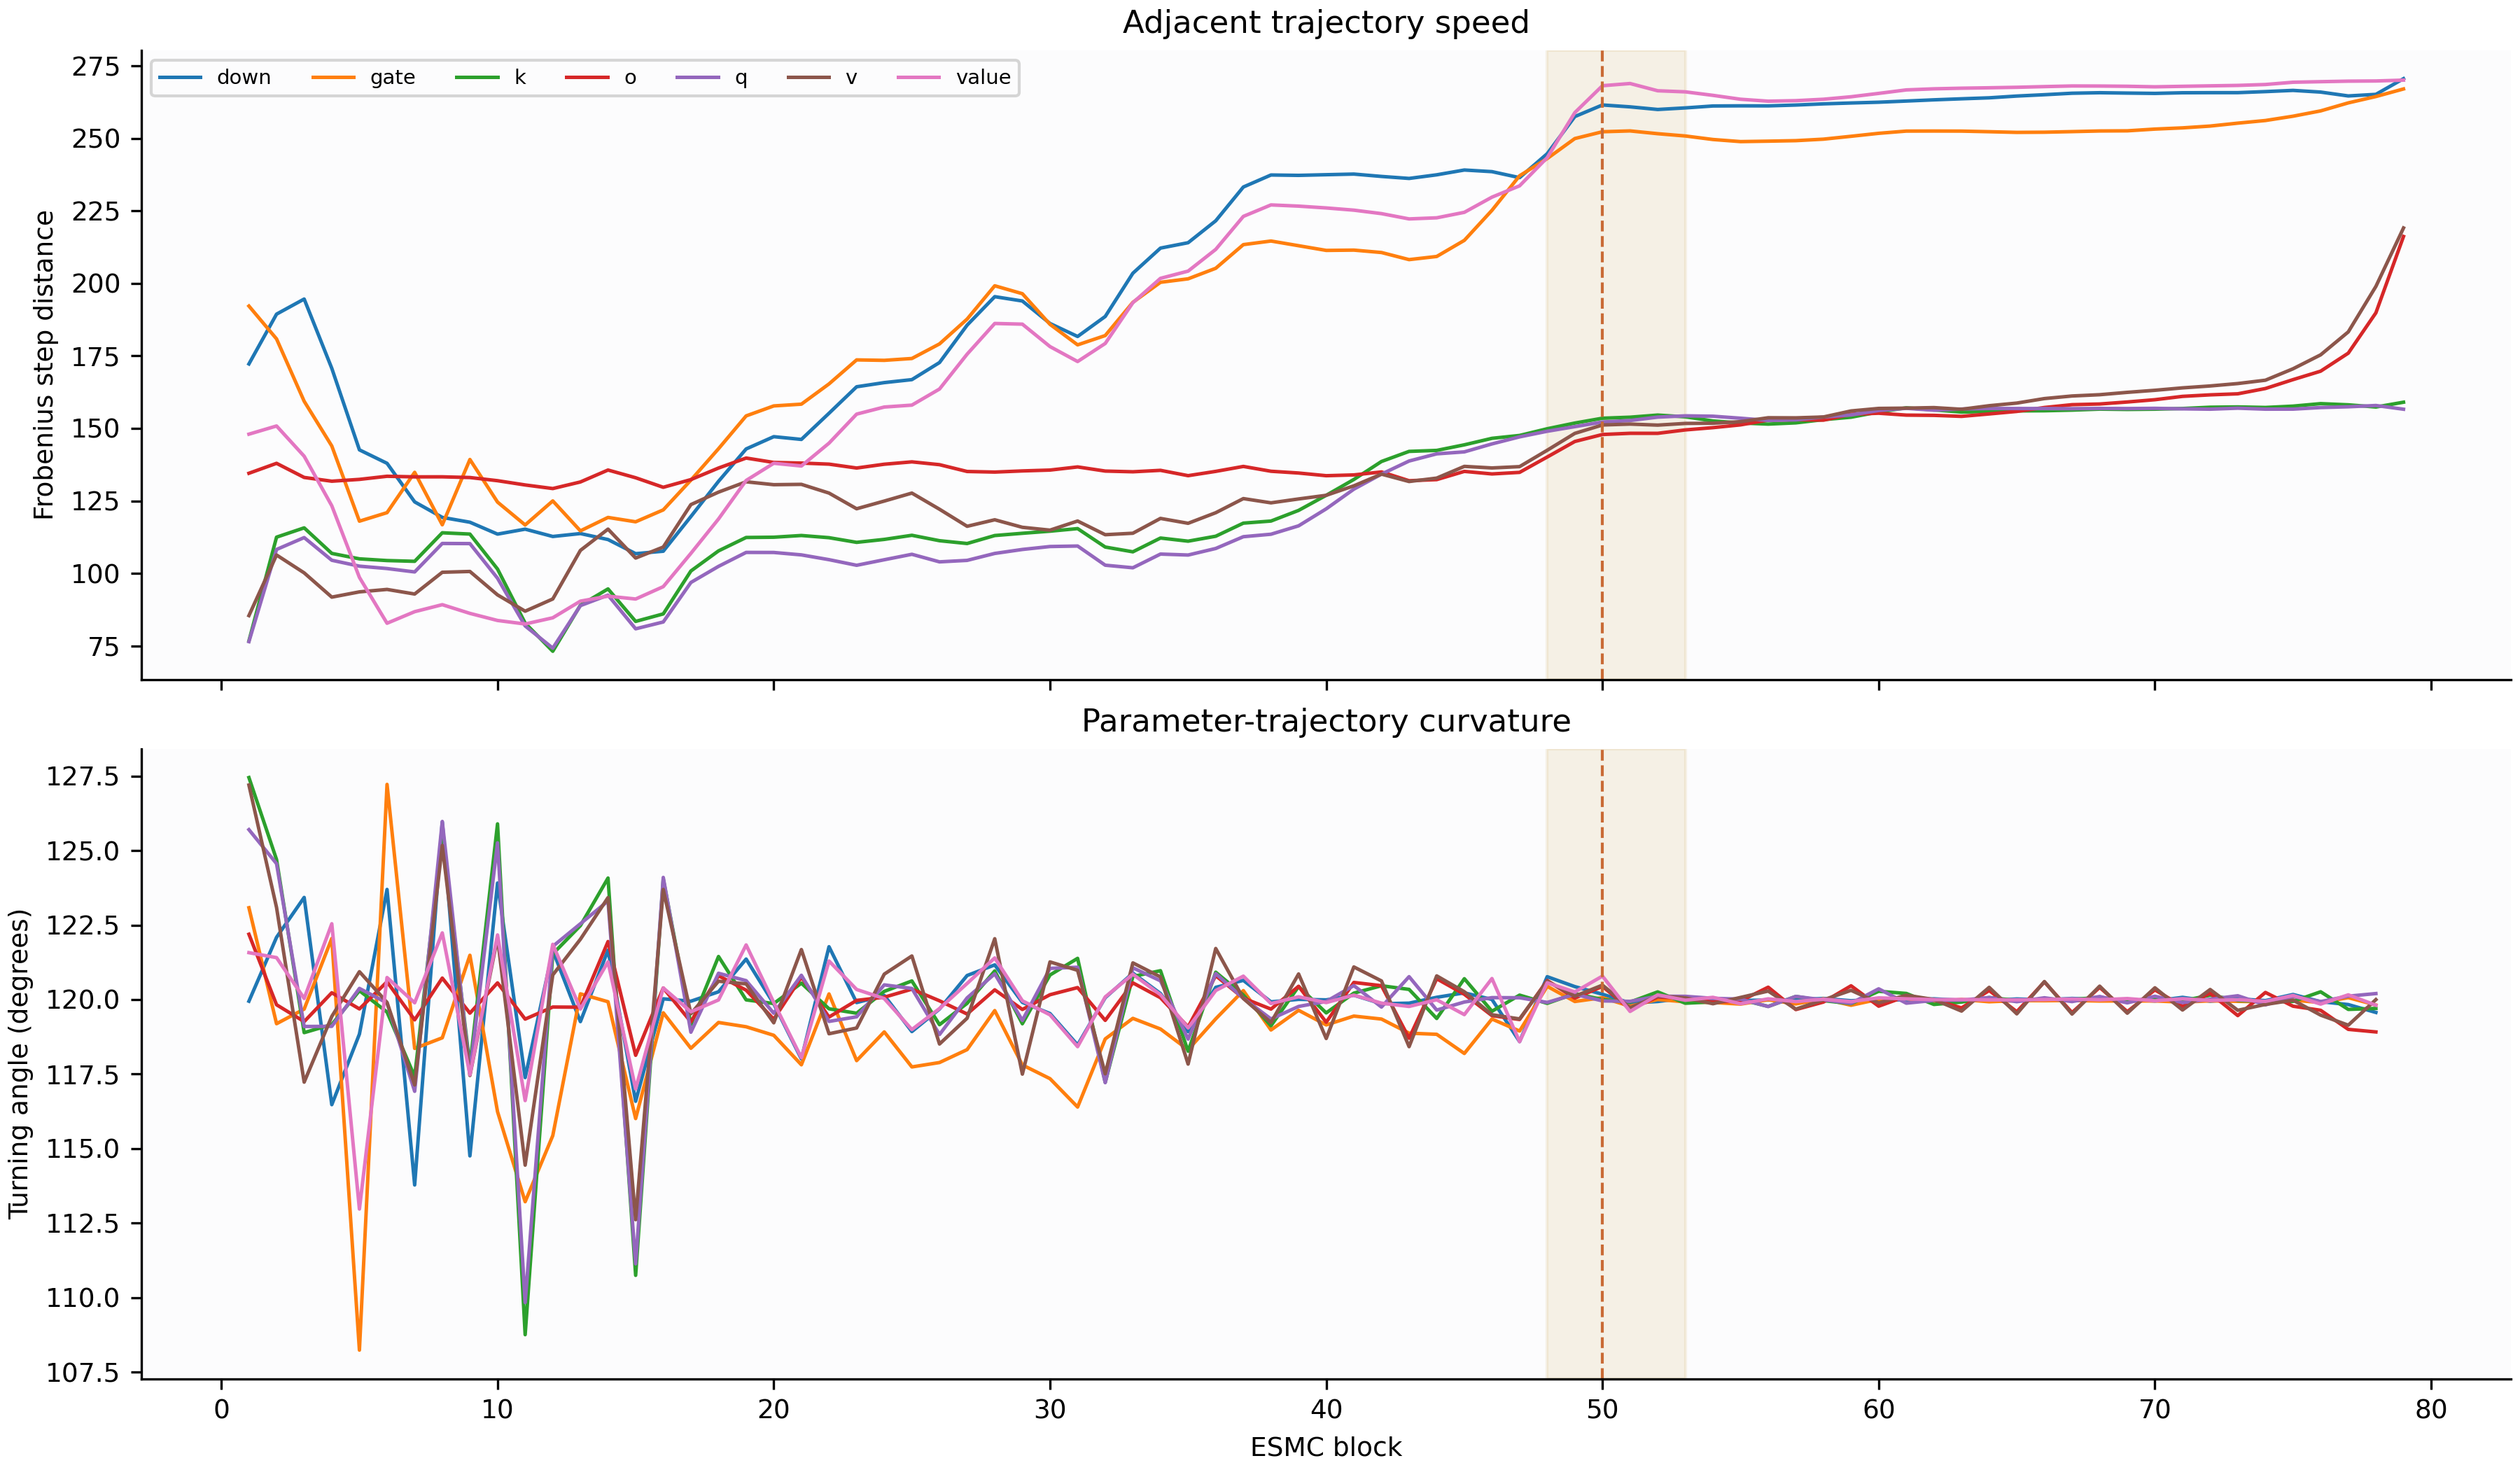
\includegraphics[width=\textwidth]{trajectory_speed_curvature.png}
\caption{Adjacent Frobenius step size and parameter-trajectory turning angle. Block 50 participates in a broader transition, but it is not the only or largest global change point.}
\label{fig:trajectory}
\end{figure}

At this stage we checked whether simpler distributional effects could account for the geometry. LayerNorm vectors were compared by mean, variance, coefficient of variation, extrema, tail quantiles, amplified and suppressed channel fractions, and adjacent-layer cosine. The closest result was the suppressed-channel fraction in the block-50 attention-input normalization at $q\approx0.052$, just outside the 5\% false-discovery threshold. More importantly, the value-projection alignment survives an explicit approximation of LayerNorm channel scaling, so a small number of unusually large or small normalization channels cannot explain the folding-readable subspace.

The raw matrix summaries in Figure~\ref{fig:raw} separate several other possibilities. Standard deviation measures the overall scale of individual weights, while excess kurtosis is zero for a Gaussian distribution and becomes large when unusually heavy tails produce more extreme weights. Row-norm Gini reuses the same inequality calculation after replacing each singular value with the Euclidean norm of one row, $x_i=\|\vect{w}_i\|_2$. A value near zero means that the rows have similar overall strength, while a large value means that a small subset of rows contains most of the matrix's magnitude. Spectral Gini and row-norm Gini therefore answer different questions. The first asks whether operator gain is concentrated in a few orthogonal directions, while the second asks whether the stored parameters are concentrated in a few output neurons. The inverse participation ratio of a unit singular vector $\vect{v}$ is
\begin{equation}
i(\vect{v})=\sum_{j=1}^{d}v_j^4.
\end{equation}
It equals $1/d$ when the vector is spread evenly across all $d$ coordinates and approaches one when it is concentrated on a single coordinate. Averaging this value across leading singular vectors tests whether the apparent subspace is broadly distributed across residual channels or localized to a few coordinates. None of these scale, tail, row-concentration, or localization summaries isolates block 50 after family-wise correction.

\begin{figure}[H]
\centering
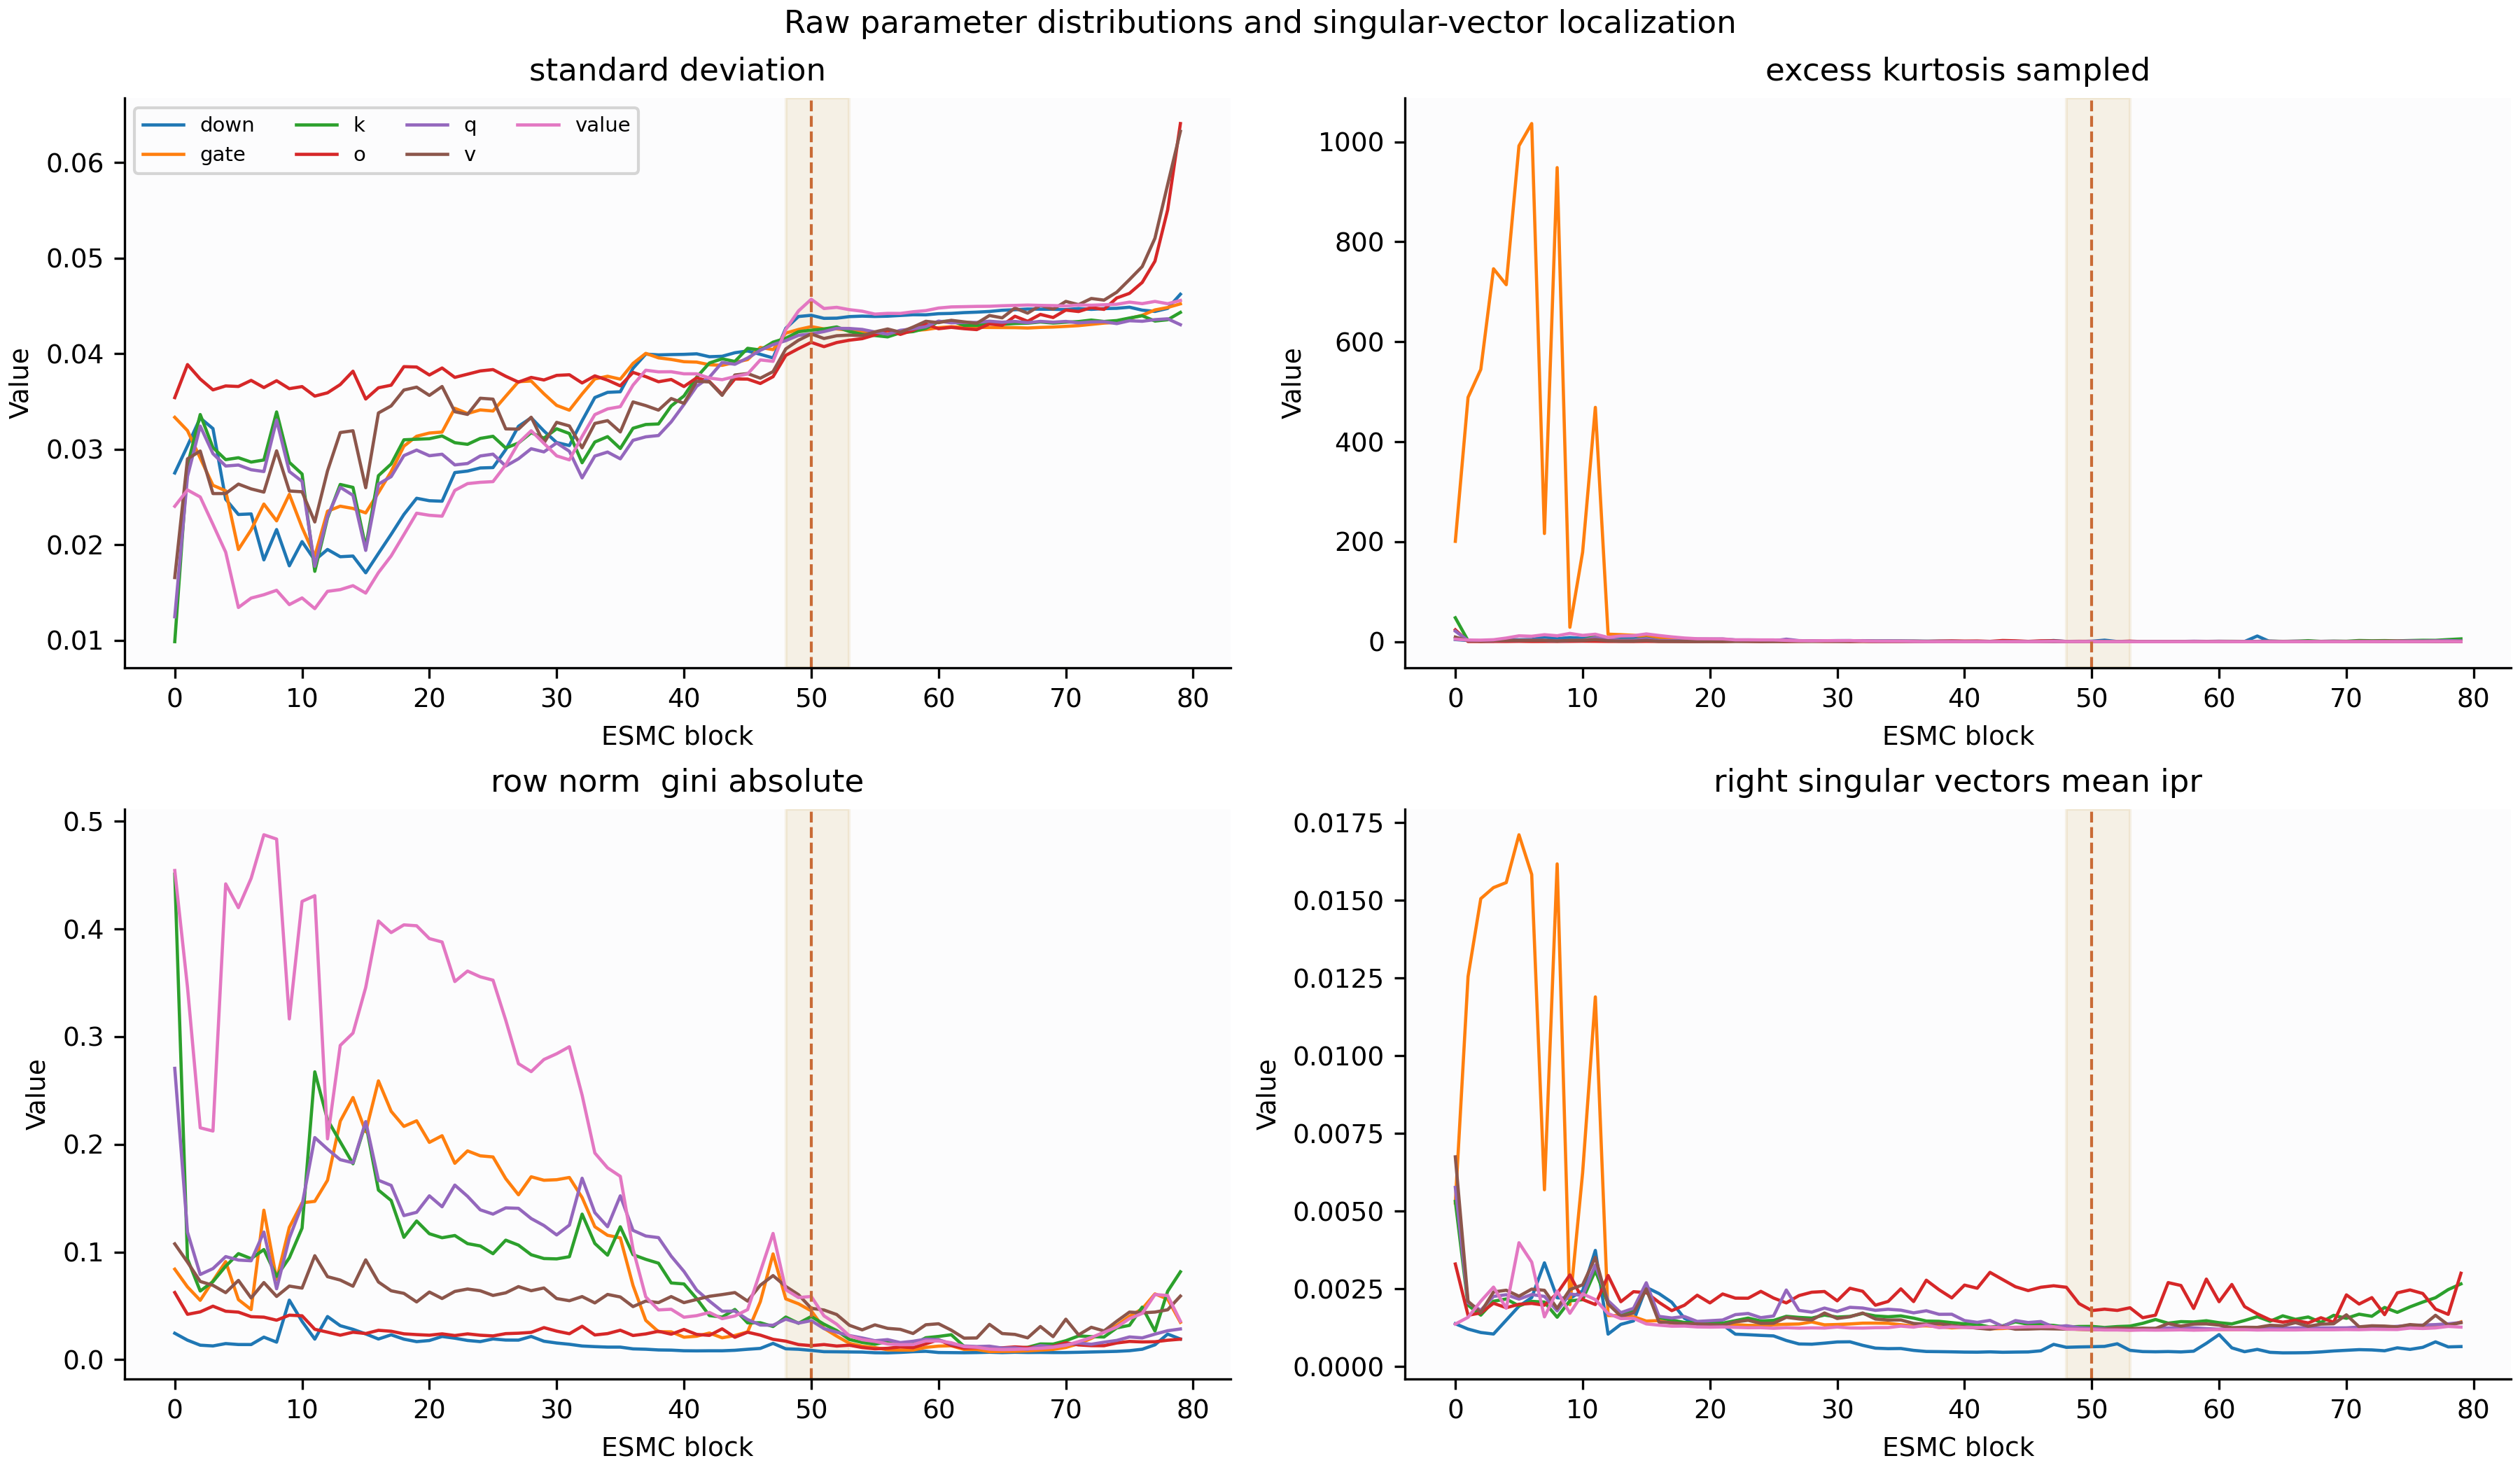
\includegraphics[width=\textwidth]{raw_parameter_profiles.png}
\caption{Raw parameter distributions and singular-vector localization. The blocks-48--53 region does not support a simple explanation based on scale, heavy tails, norm inequality, or localized singular vectors.}
\label{fig:raw}
\end{figure}

The same reasoning also motivated a compressibility control because a uniquely redundant block might tolerate more aggressive low-rank reconstruction, quantization, or pruning even if its scalar rank summaries looked ordinary. Truncated SVD uses the first $r$ singular components to produce the best rank-$r$ reconstruction under Frobenius error \cite{eckart1936}. Per-row INT8 and INT4 quantization replace each row with a smaller set of evenly spaced values whose scale is fitted to that row. Magnitude pruning removes the smallest 10\%--75\% of weights, while deterministic 2:4 pruning keeps two weights in every consecutive group of four. We compared relative Frobenius error,
\begin{equation}
\epsilon_F=\frac{\|\mat{W}-\widehat{\mat{W}}\|_F}{\|\mat{W}\|_F},
\end{equation}
along with cosine similarity, storage ratio, and spectral distortion. No block-50 or block-51 quantization or sparsity metric survives family-wise correction. Because the model was not run after compression, this result says nothing about functional tolerance. It only rules out the simpler weight-space explanation in which state 51 is selected because its producer is uniquely easy to reconstruct.

Because an 80-layer model produces smooth depth trends and thousands of related measurements, a visually striking point is not enough, so every metric was evaluated in three complementary ways. First, a cubic depth trend $f(b)$ was fitted and removed so that a late-layer value was not called unusual merely for being late,
\begin{equation}
\widetilde{x}_b=x_b-f(b).
\end{equation}
Second, local deviation was measured against the ten neighboring blocks using a robust median and median absolute deviation,
\begin{equation}
z_b^{\mathrm{local}}=0.67448975\,
\frac{x_b-\operatorname{median}(\mathcal{N}_b)}
{\operatorname{MAD}(\mathcal{N}_b)}.
\end{equation}
The constant makes the score comparable to an ordinary $z$-score for Gaussian data, while the median prevents one nearby outlier from moving the baseline too far.

Third, correlations with the mixer were tested against circular shifts. Shifting an 80-point depth profile around the circle preserves its smoothness and marginal distribution but destroys its alignment with the mixer. There are 79 nonzero shifts, so the exact smallest attainable circular-shift value is $1/80=0.0125$, while selected families also received 10,000 phase-randomized null draws. Finally, Benjamini-Hochberg correction controlled the expected false-discovery fraction within each related metric family \cite{benjamini1995}. This is why the gate overlap can be a sharp local clue at raw $p=0.0033$ but remain supporting evidence at $q=0.132$, while the value overlap survives as the cleaner result.

\begin{figure}[H]
\centering
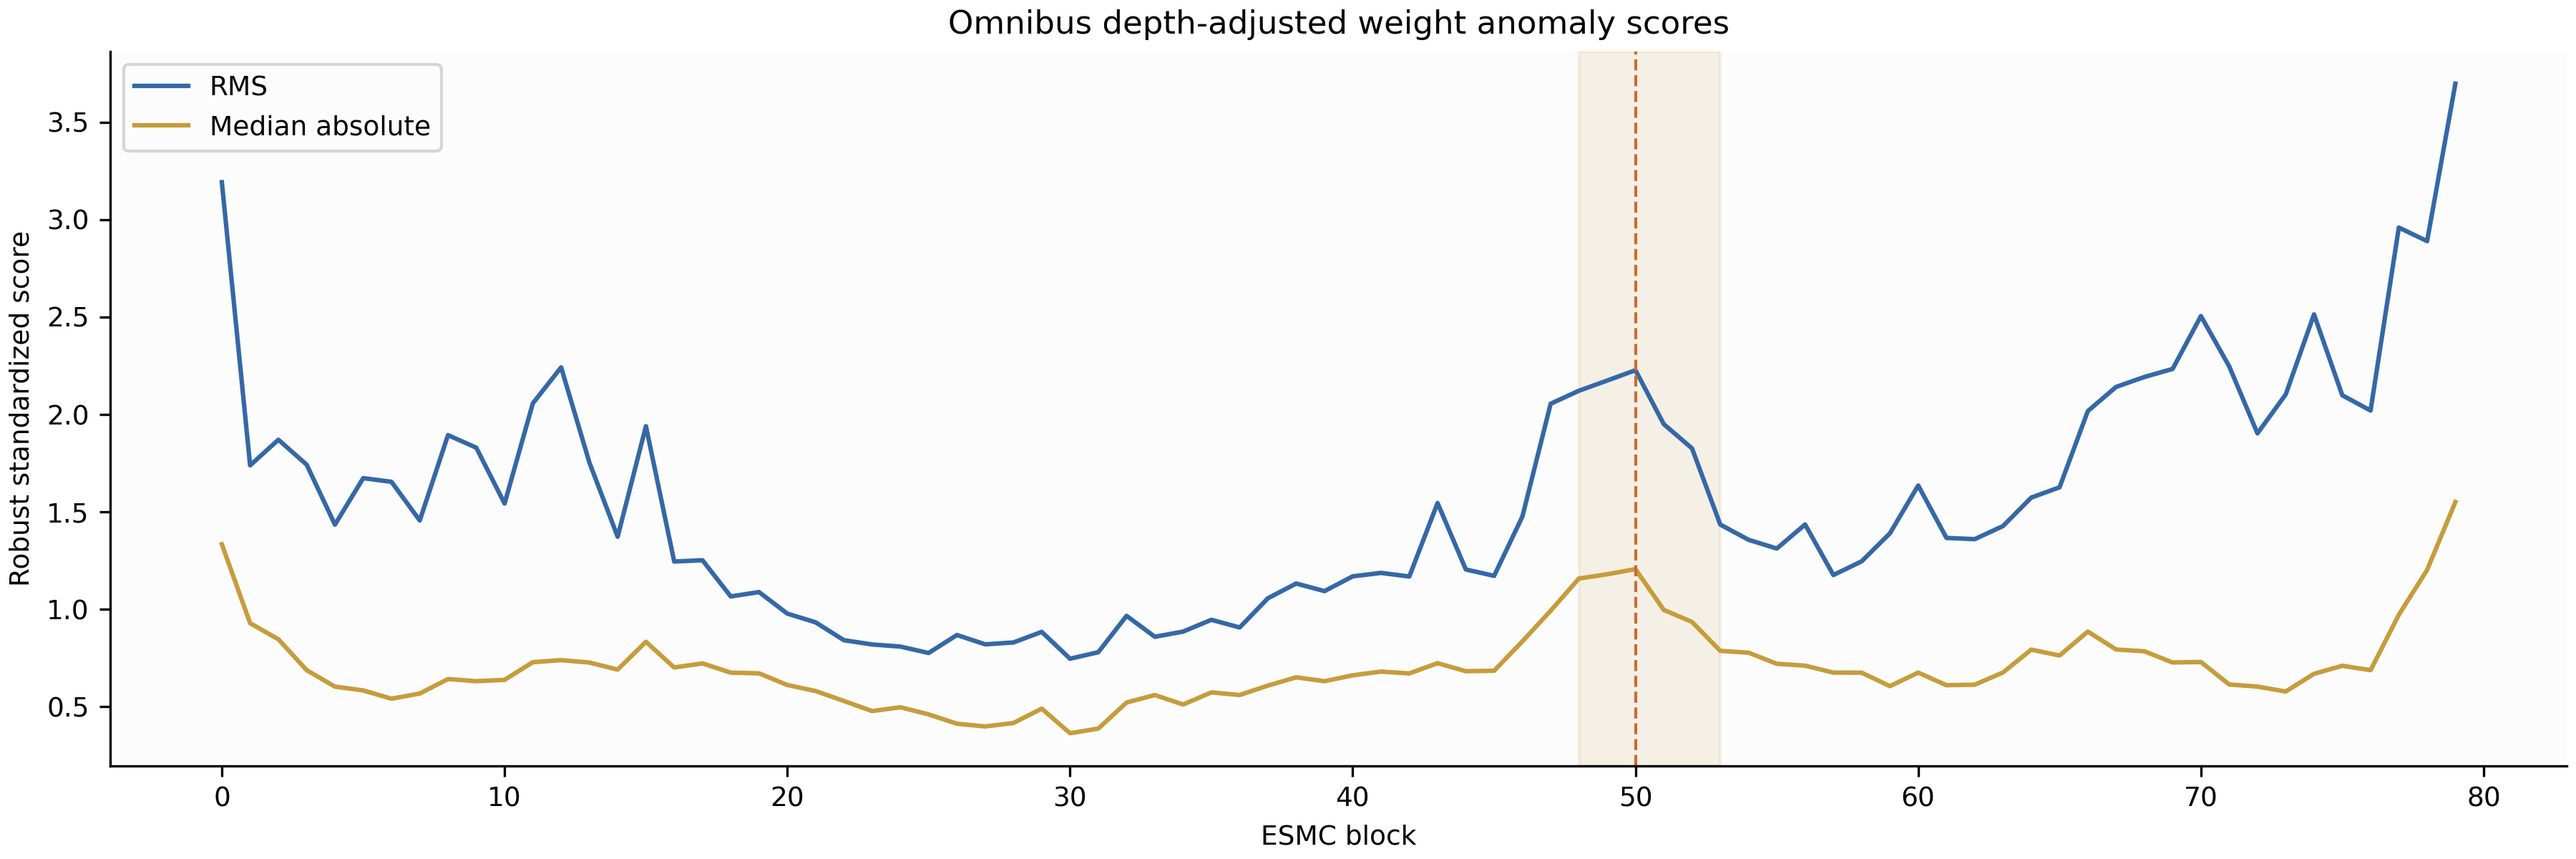
\includegraphics[width=\textwidth]{layer_omnibus_anomalies.png}
\caption{Omnibus depth-adjusted anomaly scores. Blocks 48--53 form an elevated local regime and block 50 is prominent within it, although late blocks also contain large global weight anomalies.}
\label{fig:omnibus}
\end{figure}

The numerical checks matter because Gram methods square the condition number and can exaggerate small floating-point errors. Direct FP32 SVD on blocks 0, 50, 51, and 79 differs from the FP64 Gram spectrum by at most $4.48\times10^{-4}$ across the leading 64 singular values. The retained squared-magnitude fraction differs by at most $6.29\times10^{-4}$, and the ranks needed to reach 90\%, 95\%, and 99\% differ by at most one. Randomized rank-64 bases are less stable, with a worst leading-spectrum difference of 10.2\% and minimum replicate subspace overlap 0.526, so none of the inferential claims depends on those randomized bases, and all 64 saved output-quality checks passed.

Putting the measurements together makes the original discrepancy easier to interpret. The final states dominate the \ESMFold mixture because they expose the strongest broadly accessible tertiary-structure signal, which accounts for the positive P@L-to-mixer correlation across depth. State 51 departs from that relationship because block 50 appears to create a locally unusual interface to the folding reader while the network is moving through a broader transition spanning blocks 48--53. Several attention heads become strongly read/write coupled in the same block, their roles reorganize across the neighboring layers, and the SwiGLU gate and value spaces become unusually aligned with the folding projection. At the same time, the down pathway spreads neuron-wise coupling into stronger positive and negative tails. None of the whole-matrix tests indicates that block 50 is globally low-rank, globally more complex, or uniquely compressible. Its distinction is relative to the geometry of the downstream projection.

This gives layer importance a more useful interpretation than a single maximum of ``information.'' A transformer state can matter because it forms a temporary interface in which one block writes a computation using coordinates that a downstream module recognizes. Later blocks can rewrite those coordinates while continuing to improve other capabilities. Contact probes, sparse autoencoders, masked-language-model perplexity, and folding projections can then disagree without any measurement being defective, since each one uses a different operation to select directions from the state.

In mechanistic-interpretability terms, the weights identify an available circuit in which attention provides a distributed relay, the FFN consolidates and writes a compact component, state 51 exposes that component, and the shared \ESMFold projection is positioned to select it \cite{olah2020}. This interpretation is stronger than a coincident peak in two depth profiles because it links consecutive operators in the same residual coordinate system and survives controls for scale, depth, normalization, and multiple testing. The evidence remains weights-only, however, so it cannot show that real protein activations occupy the aligned subspace, that the coupled heads operate together on a particular fold, or that removing the component damages structure prediction.

The most direct causal test would remove the rank-16 component of the block-50 value subspace that aligns with the folding projection, then compare the intervention with equal-rank and equal-norm components chosen from the orthogonal complement. Folding quality, P@L, SAE reconstruction, and masked-language-model behavior should be measured together. A selective loss of folding performance would show that \ESMFold actually uses the route identified by the weights. Until that intervention is performed, the supported conclusion is narrower. Block 50 appears to write a transient projection-aligned folding interface, and \ESMFold assigns substantial weight to state 51 because that is the state in which the interface is available to its shared reader.

All weight calculations used the pinned Biohub \ESMC revision cited below
\cite{biohub2026}. Its full revision identifier was
\begin{center}
\small\texttt{45b0fa5d7fb06faefbd5e3b89bdcef35d564e79a}.
\end{center}
All six safetensor shard hashes were verified, matrices were streamed without
instantiating \ESMC, and computation ran on an NVIDIA GH200 480GB workstation
with CUDA 12.8 and Python 3.10.12. The four \ESMFold checkpoints contributed
only their mixing logits, shared folding LayerNorm, and shared
$2560\rightarrow256$ projection. Token embeddings, the masked-language-model
head, the folding trunk, and the structure module were outside the primary
weight analysis.

\clearpage
\begin{thebibliography}{12}

\bibitem{candido2026}
S. Candido, T. Hayes, A. Derry, et al.
``Language Modeling Materializes a World Model of Protein Biology.''
\textit{bioRxiv}, 2026.06.03.729735, 2026.
\url{https://doi.org/10.64898/2026.06.03.729735}.

\bibitem{rives2021}
A. Rives, J. Meier, T. Sercu, et al.
``Biological structure and function emerge from scaling unsupervised learning to 250 million protein sequences.''
\textit{Proceedings of the National Academy of Sciences}, 118(15):e2016239118, 2021.
\url{https://doi.org/10.1073/pnas.2016239118}.

\bibitem{rao2021}
R. Rao, J. Meier, T. Sercu, S. Ovchinnikov, and A. Rives.
``Transformer protein language models are unsupervised structure learners.''
\textit{International Conference on Learning Representations}, 2021.
\url{https://openreview.net/forum?id=fylclEqgvgd}.

\bibitem{lin2023}
Z. Lin, H. Akin, R. Rao, et al.
``Evolutionary-scale prediction of atomic-level protein structure with a language model.''
\textit{Science}, 379(6637):1123--1130, 2023.
\url{https://doi.org/10.1126/science.ade2574}.

\bibitem{facco2017}
E. Facco, M. d'Errico, A. Rodriguez, and A. Laio.
``Estimating the intrinsic dimension of datasets by a minimal neighborhood information.''
\textit{Scientific Reports}, 7:12140, 2017.
\url{https://doi.org/10.1038/s41598-017-11873-y}.

\bibitem{levina2004}
E. Levina and P. J. Bickel.
``Maximum Likelihood Estimation of Intrinsic Dimension.''
\textit{Advances in Neural Information Processing Systems}, 17, 2004.
\url{https://papers.nips.cc/paper/2004/hash/74934548253bcab8490ebd74afed7031-Abstract.html}.

\bibitem{benjamini1995}
Y. Benjamini and Y. Hochberg.
``Controlling the False Discovery Rate: A Practical and Powerful Approach to Multiple Testing.''
\textit{Journal of the Royal Statistical Society: Series B}, 57(1):289--300, 1995.
\url{https://doi.org/10.1111/j.2517-6161.1995.tb02031.x}.

\bibitem{eckart1936}
C. Eckart and G. Young.
``The approximation of one matrix by another of lower rank.''
\textit{Psychometrika}, 1:211--218, 1936.
\url{https://doi.org/10.1007/BF02288367}.

\bibitem{kuhn1955}
H. W. Kuhn.
``The Hungarian method for the assignment problem.''
\textit{Naval Research Logistics Quarterly}, 2(1--2):83--97, 1955.
\url{https://doi.org/10.1002/nav.3800020109}.

\bibitem{olah2020}
C. Olah, N. Cammarata, L. Schubert, G. Goh, M. Petrov, and S. Carter.
``Zoom In: An Introduction to Circuits.''
\textit{Distill}, 2020.
\url{https://doi.org/10.23915/distill.00024.001}.

\bibitem{roy2007}
O. Roy and M. Vetterli.
``The effective rank: A measure of effective dimensionality.''
\textit{15th European Signal Processing Conference}, pages 606--610, 2007.

\bibitem{biohub2026}
Biohub.
\textit{ESMC-6B checkpoint}, revision
\texttt{45b0fa5d7fb06faefbd5e3b89bdcef35d564e79a}.
\url{https://huggingface.co/biohub/ESMC-6B}.

\end{thebibliography}

\end{document}
